\documentclass[a4paper]{article}
\usepackage[pdftex]{hyperref}
\usepackage[latin1]{inputenc}
\usepackage[english]{babel}
\usepackage{a4wide}
\usepackage{amsmath}
\usepackage{amssymb}
\usepackage{algorithmic}
\usepackage{algorithm}
\usepackage{ifthen}
\usepackage{listings}
% move the asterisk at the right position
\lstset{basicstyle=\ttfamily,tabsize=4,literate={*}{${}^*{}$}1}
%\lstset{language=C,basicstyle=\ttfamily}
\usepackage{moreverb}
\usepackage{palatino}
\usepackage{multicol}
\usepackage{tabularx}
\usepackage{comment}
\usepackage{verbatim}
\usepackage{color}

%% pdflatex?
\newif\ifpdf
\ifx\pdfoutput\undefined
\pdffalse % we are not running PDFLaTeX
\else
\pdfoutput=1 % we are running PDFLaTeX
\pdftrue
\fi
\ifpdf
\usepackage[pdftex]{graphicx}
\else
\usepackage{graphicx}
\fi
\ifpdf
\DeclareGraphicsExtensions{.pdf, .jpg}
\else
\DeclareGraphicsExtensions{.eps, .jpg}
\fi

\parindent=0cm
\parskip=0cm

\setlength{\columnseprule}{0.4pt}
\addtolength{\columnsep}{2pt}

\addtolength{\textheight}{5.5cm}
\addtolength{\topmargin}{-26mm}
\pagestyle{empty}

%%
%% Sheet setup
%% 
\newcommand{\coursename}{Image Processing}
\newcommand{\courseno}{CAS-320321}
 
\newcommand{\sheettitle}{Homework}
\newcommand{\mytitle}{}
\newcommand{\mytoday}{{February 20}, 2020}

% Current Assignment number
\newcounter{assignmentno}
\setcounter{assignmentno}{1}

% Current Problem number, should always start at 1
\newcounter{problemno}
\setcounter{problemno}{1}

%%
%% problem and bonus environment
%%
\newcounter{probcalc}
\newcommand{\problem}[2]{
  \pagebreak[2]
  \setcounter{probcalc}{#2}
  ~\\
  {\large \textbf{Problem {\arabic{assignmentno}}.{\arabic{problemno}}} \hspace{0.2cm}\textit{#1}} \refstepcounter{problemno}\vspace{2pt}\\}

\newcommand{\bonus}[2]{
  \pagebreak[2]
  \setcounter{probcalc}{#2}
  ~\\
  {\large \textbf{Bonus Problem {\arabic{assignmentno}}.{\arabic{problemno}}} \hspace{0.2cm}\textit{#1}} \refstepcounter{problemno}\vspace{2pt}\\}

%% some counters  
\newcommand{\assignment}{\arabic{assignmentno}}

%% solution  
\newcommand{\solution}{\pagebreak[2]{\bf Solution:}\\}

%% Hyperref Setup
\hypersetup{pdftitle={Homework \assignment},
  pdfsubject={\coursename},
  pdfauthor={},
  pdfcreator={},
  pdfkeywords={Computer Architecture and Programming Languages},
  %  pdfpagemode={FullScreen},
  %colorlinks=true,
  %bookmarks=true,
  %hyperindex=true,
  bookmarksopen=false,
  bookmarksnumbered=true,
  breaklinks=true,
  %urlcolor=darkblue
  urlbordercolor={0 0 0.7}
}

\begin{document}
\coursename \hfill Course: \courseno\\
Jacobs University Bremen \hfill \mytoday\\
{Otmane Sabir}\hfill \\
{Aadil Anil Kumar}\hfill
\vspace*{0.3cm}\\
\begin{center}
{\Large \sheettitle{} {\assignment}\\}
\end{center}

\large\texbf{General Information} \\
?????\\

\large\texbf{Experiment 1: Symmetric vs. Asymmetric SE on f3} \\ 
\begin{figure}[htp]
    \centering
    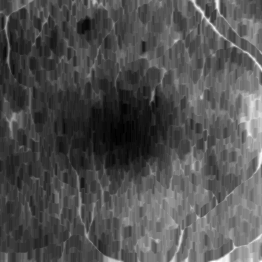
\includegraphics[width=6cm]{eroSym.png}
    \caption{Erosion with Symmetric SE}
    \label{fig:erosionSym}
\end{figure}
\begin{figure}[htp]
    \centering
    \includegraphics[width=6cm]{eroAsym.png}
    \caption{Erosion with Asymmetric SE}
    \label{fig:erosionAsym}
\end{figure}

The symmetric structuring element that we chose for eroding the image f3 was a backward diagonal of size 9 (SE5.txt). Figure 1 depicts this result. \\

The asymmetric structuring element that we chose for the same operation was a 9x10 that closely resembles a backward diagonal (SE7.txt). \\\

As expected when using an asymmetric SE, the chosen border handling method does introduce an artifact to the image. If you were to observe and compare Figure 1 and 2 closely you can see that the bottom border of Figure 2 contains a row of white space. This is easier to see when viewing the image with a black background. \\

\newpage
\large\texbf{} \\ 


\end{document}